\subsection{INTEGER type}

The \textit{INTEGER} type is design as 8 bytes $({b} = 8)$, but for easy to explain the \textit{INTEGER} type design in Li's Hash, so the example below which will explain in 4 bytes $(b = 4)$.\\

As normal integer, the \textit{INTEGER} type can be also signed and unsigned, this information will record in the metadata, so this will not show in index table, the different between them is the operation have a little bit different, but they share the same index table. Same as the \textit{BOOLEAN} type, the invert index table is not needed. Because of the inverted index table cost spaces but don't provide a significant speed up for the operation.\\

We use figure \ref{fig:algorithm:integer:example_1} to explain these operations below:

\begin{figure}[h]
\centering
%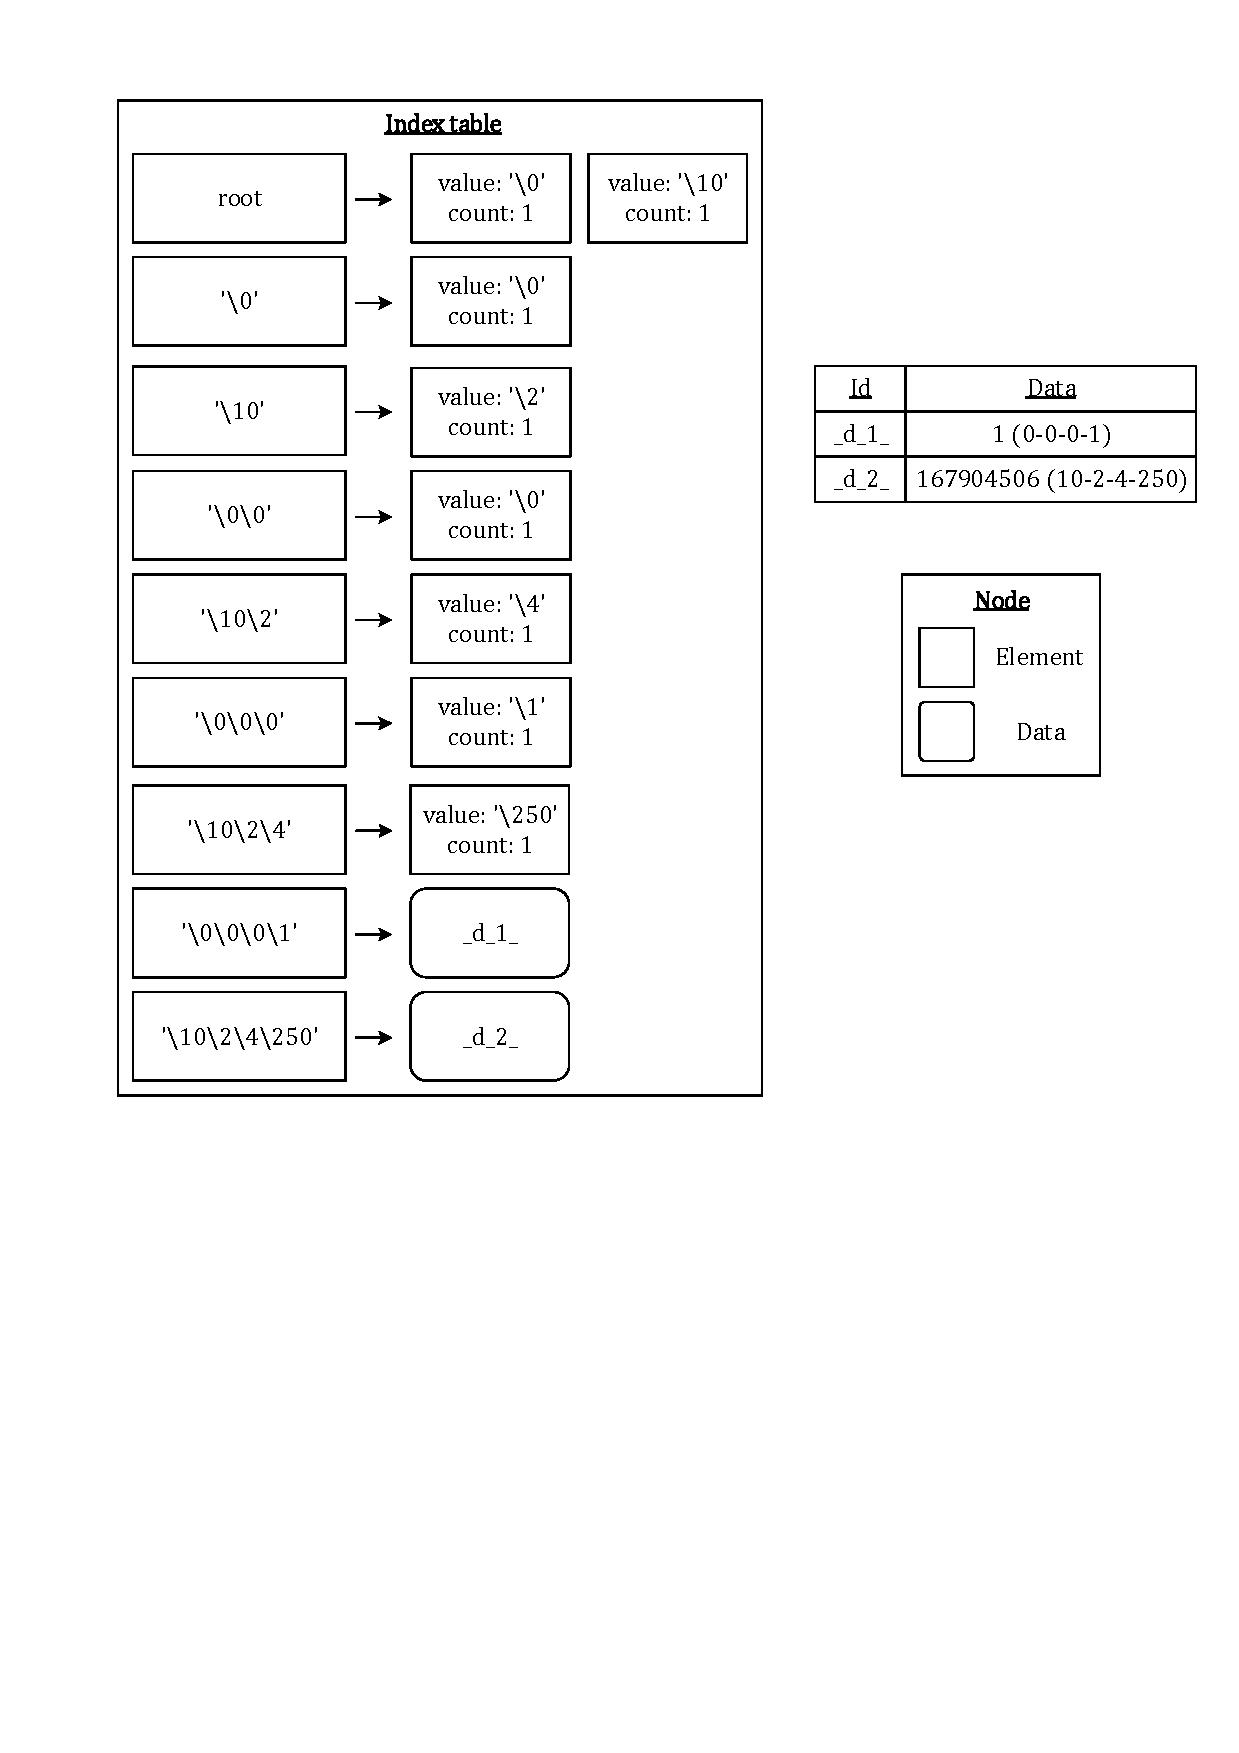
\includegraphics[scale=0.45]{./algorithm/integer/pic/example_1_v3.pdf}
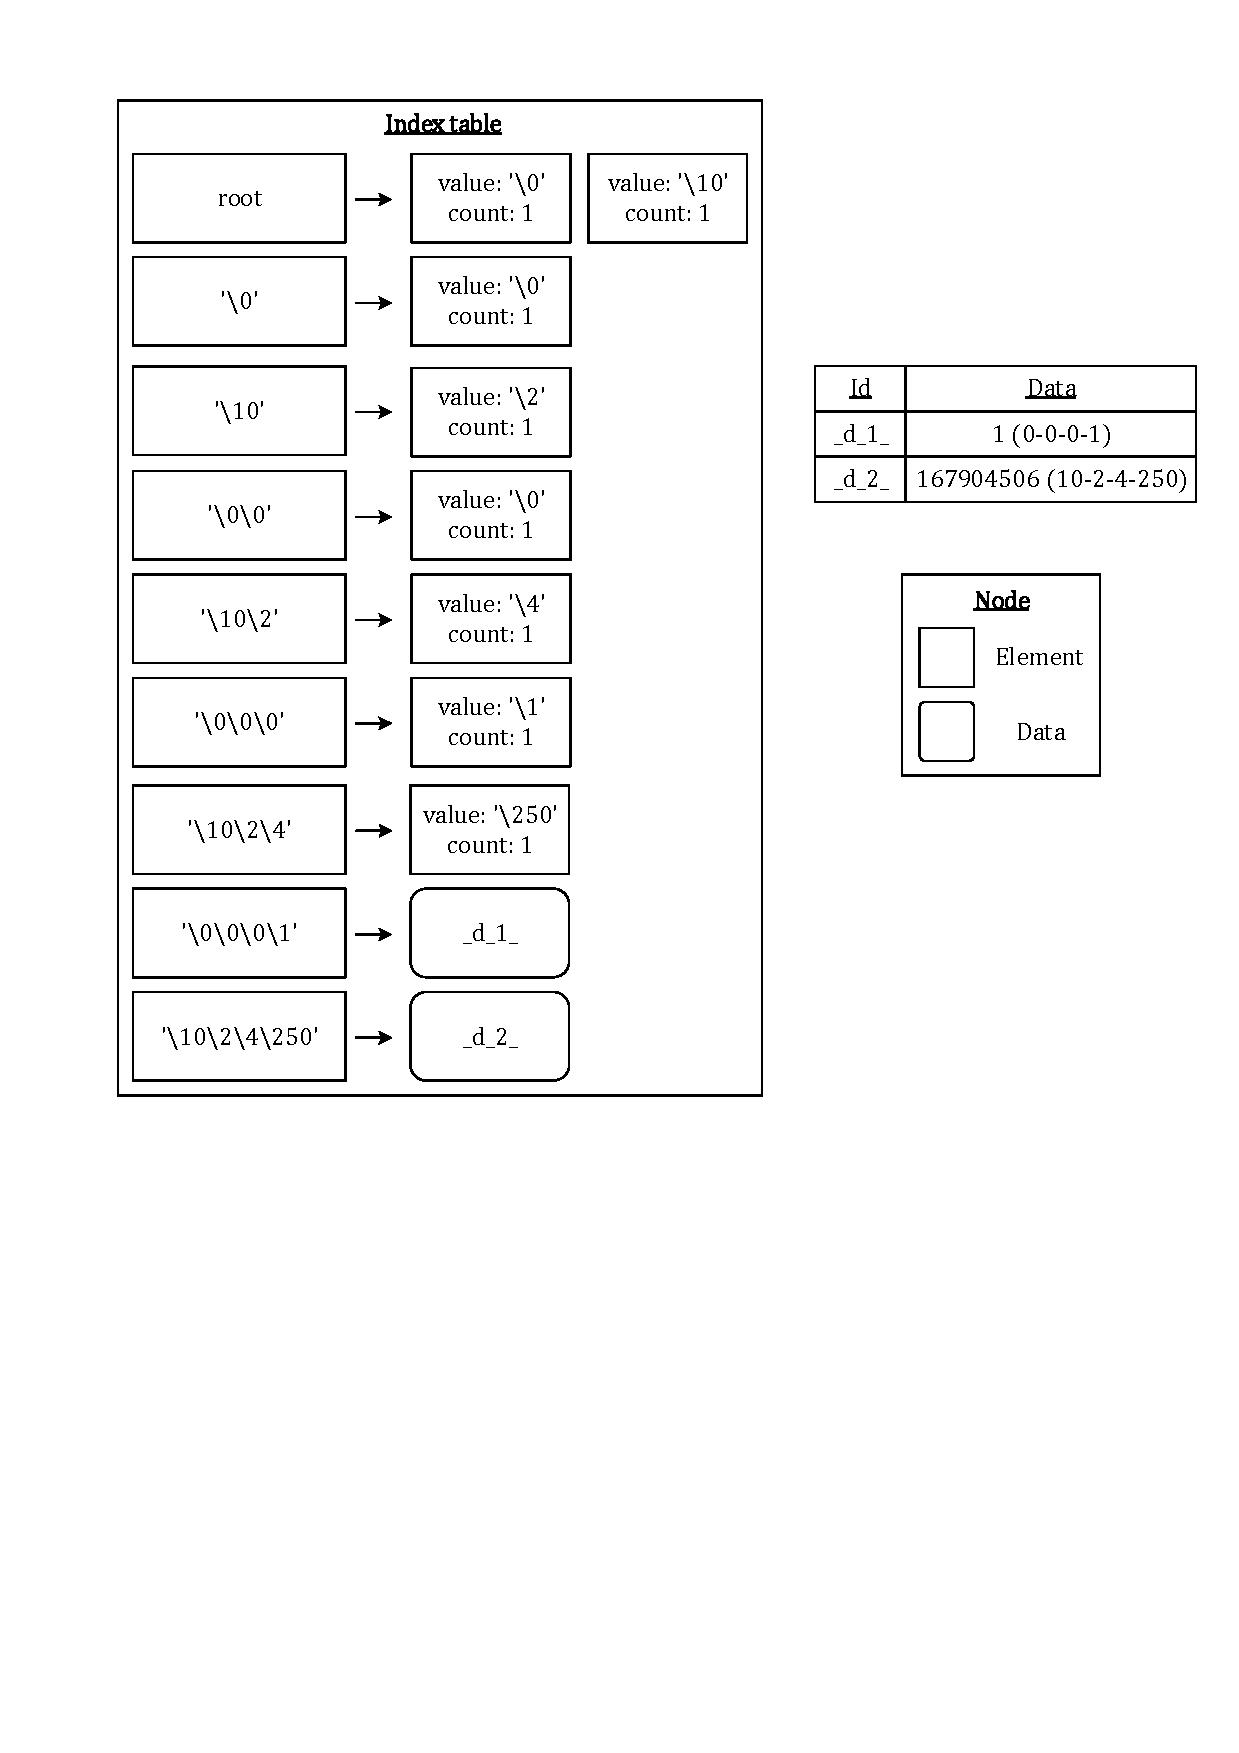
\includegraphics[width=0.8\textwidth]{./algorithm/integer/pic/example_1_v3.pdf}
\caption{The indexing tables of \textit{INTEGER} type.}
\label{fig:algorithm:integer:example_1}
\end{figure}

The index table is start with a root key \textit{'root'}. The root key is use to record the first byte of the data, so it will point to the range of 0 to 255.\\

In figure \ref{fig:algorithm:integer:example_1}, there are two data in the table. The four bytes of \textit{1} is \textit{0-0-0-1}, and \textit{167904506} is \textit{10-2-4-250} in byte. So in the table, the \textit{'root'} is pointing to \textit{'$\backslash0$'} and \textit{'$\backslash10$'}. After root key is finish its' indexing, the next step is just using n-gram indexing to index remain bytes to store data in the table.\\


% Insertion section
\subsubsection{Insertion}

Figure \ref{fig:algorithm:integer:example_1} already described some of the flow of insertion, so in here will show the table if insert a negative value into the table. Insert a -2147483647 (128-0-0-1) into table, which will become like figure \ref{fig:algorithm:integer:insertion:example_1}.

\begin{figure}[h]
\centering
%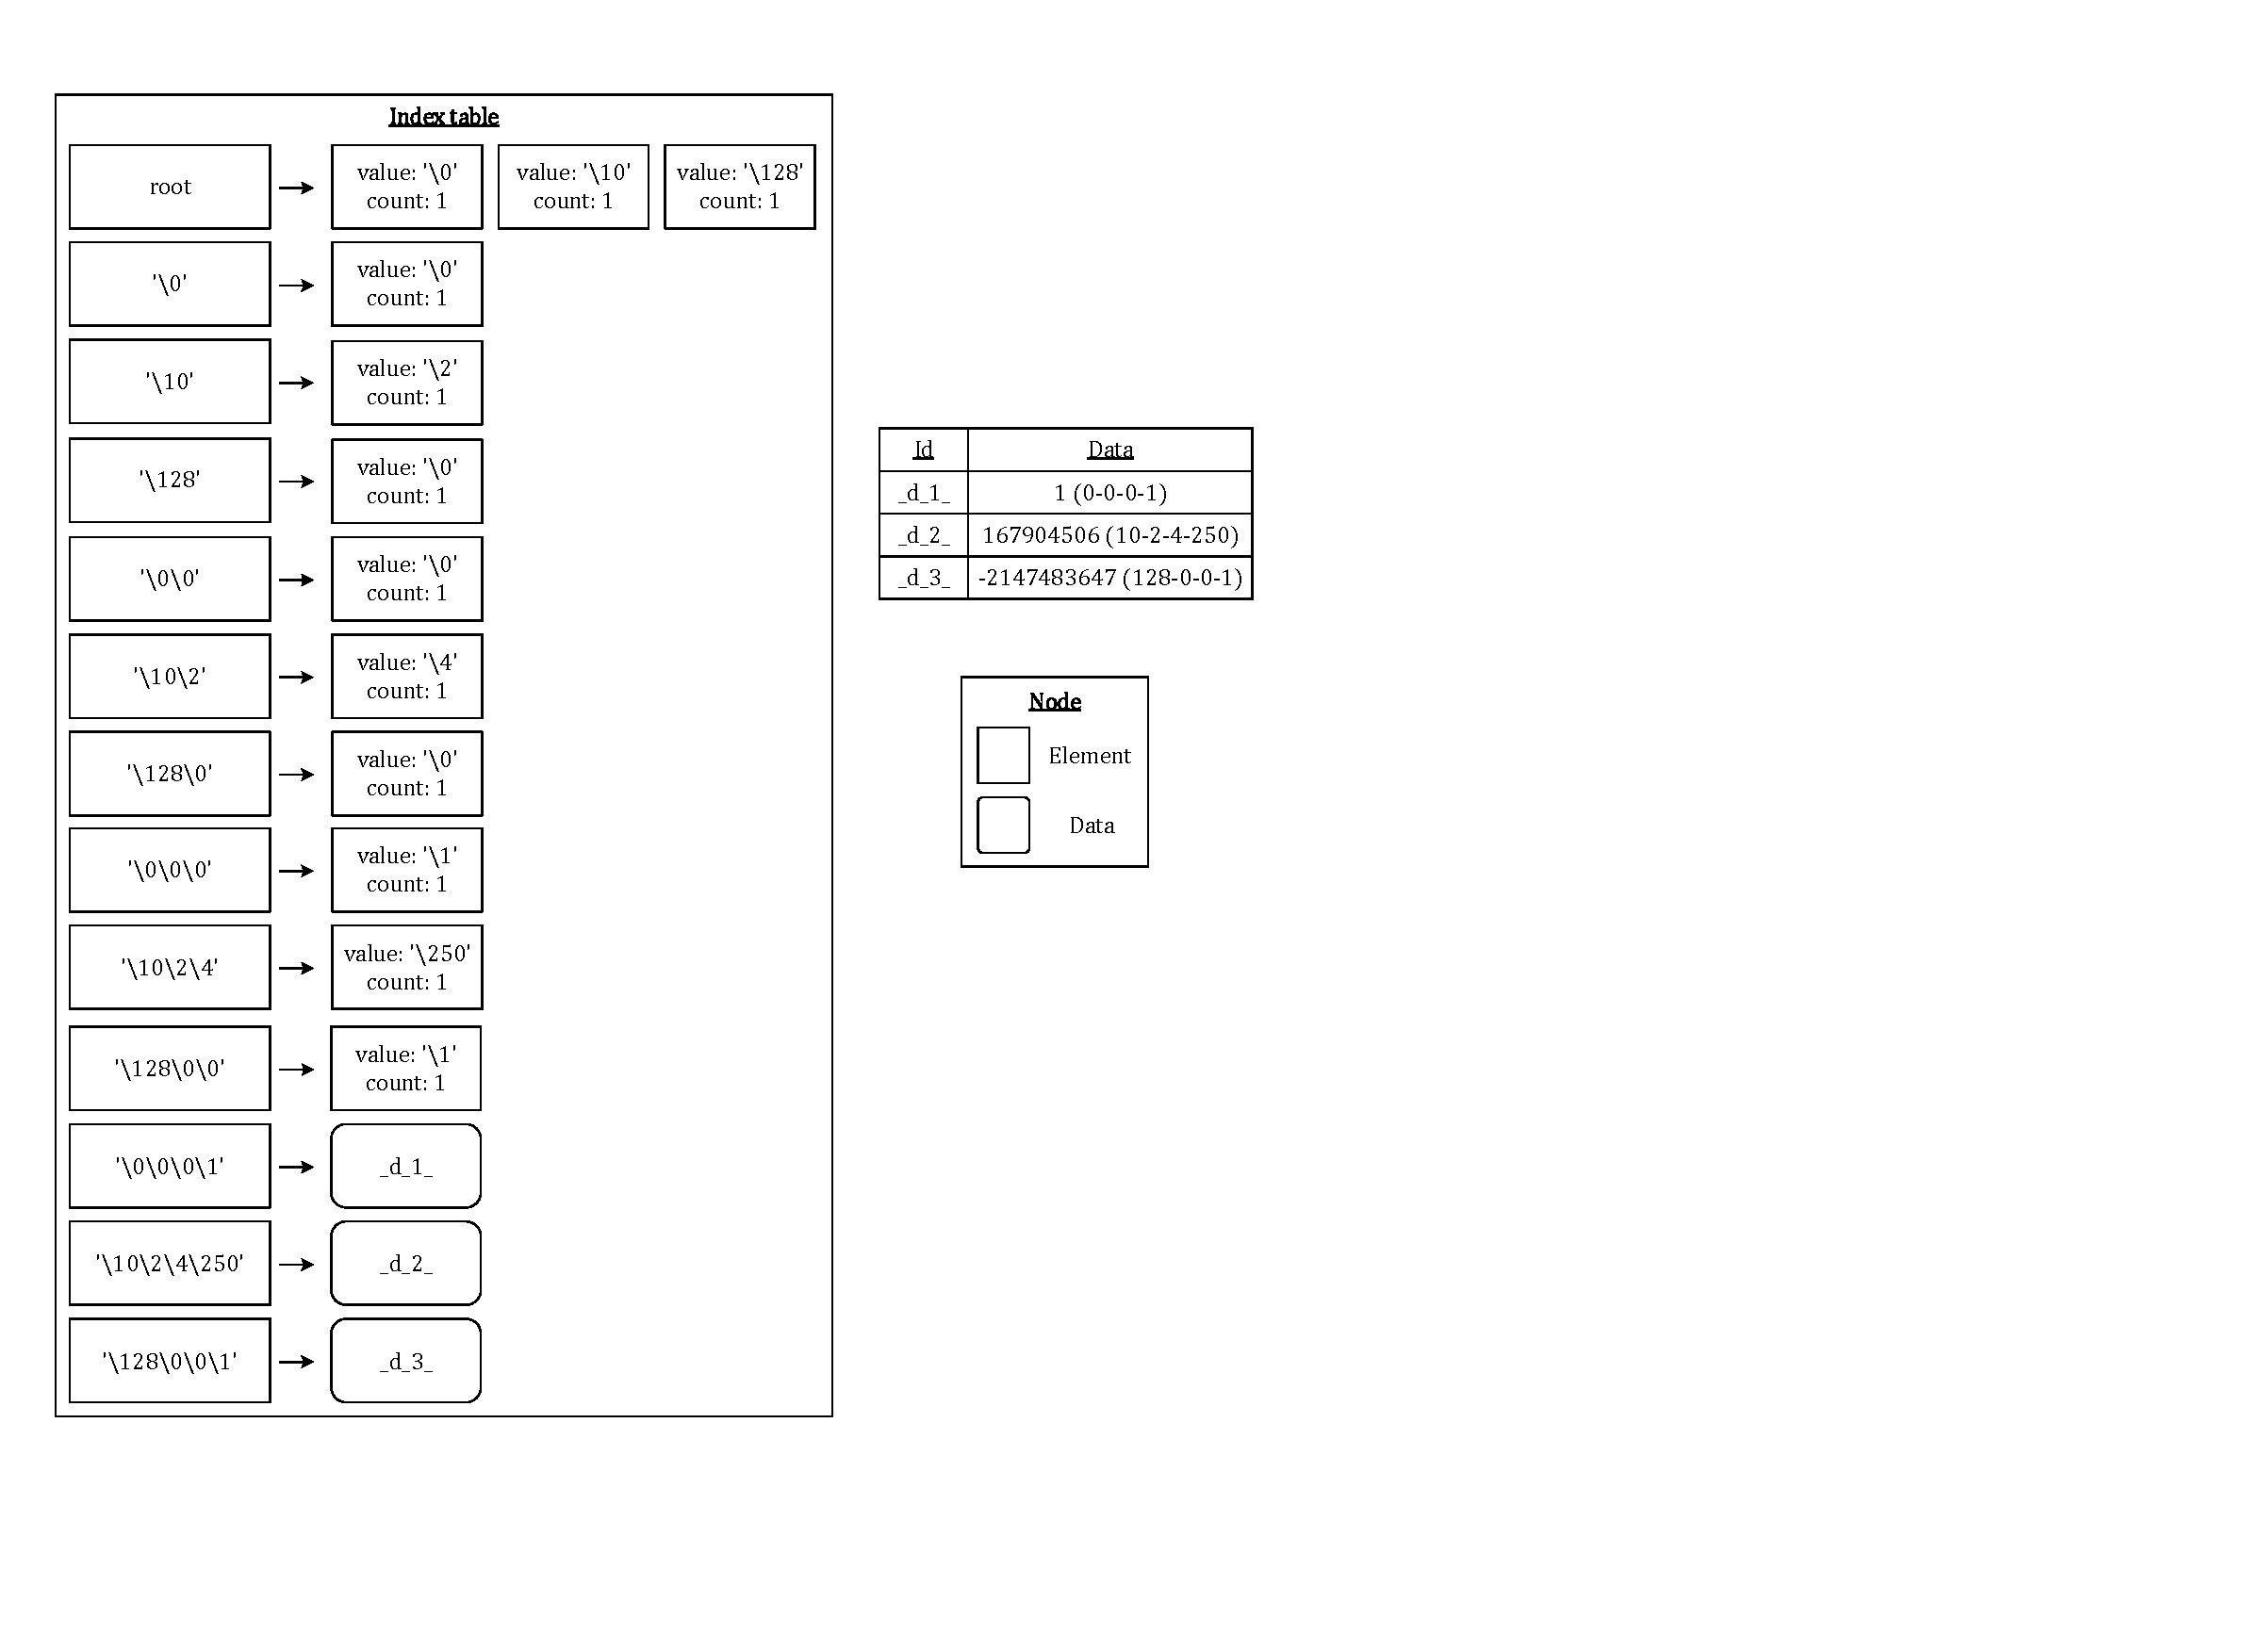
\includegraphics[scale=0.6]{./algorithm/integer/pic/insertion/example_1_v3.pdf}
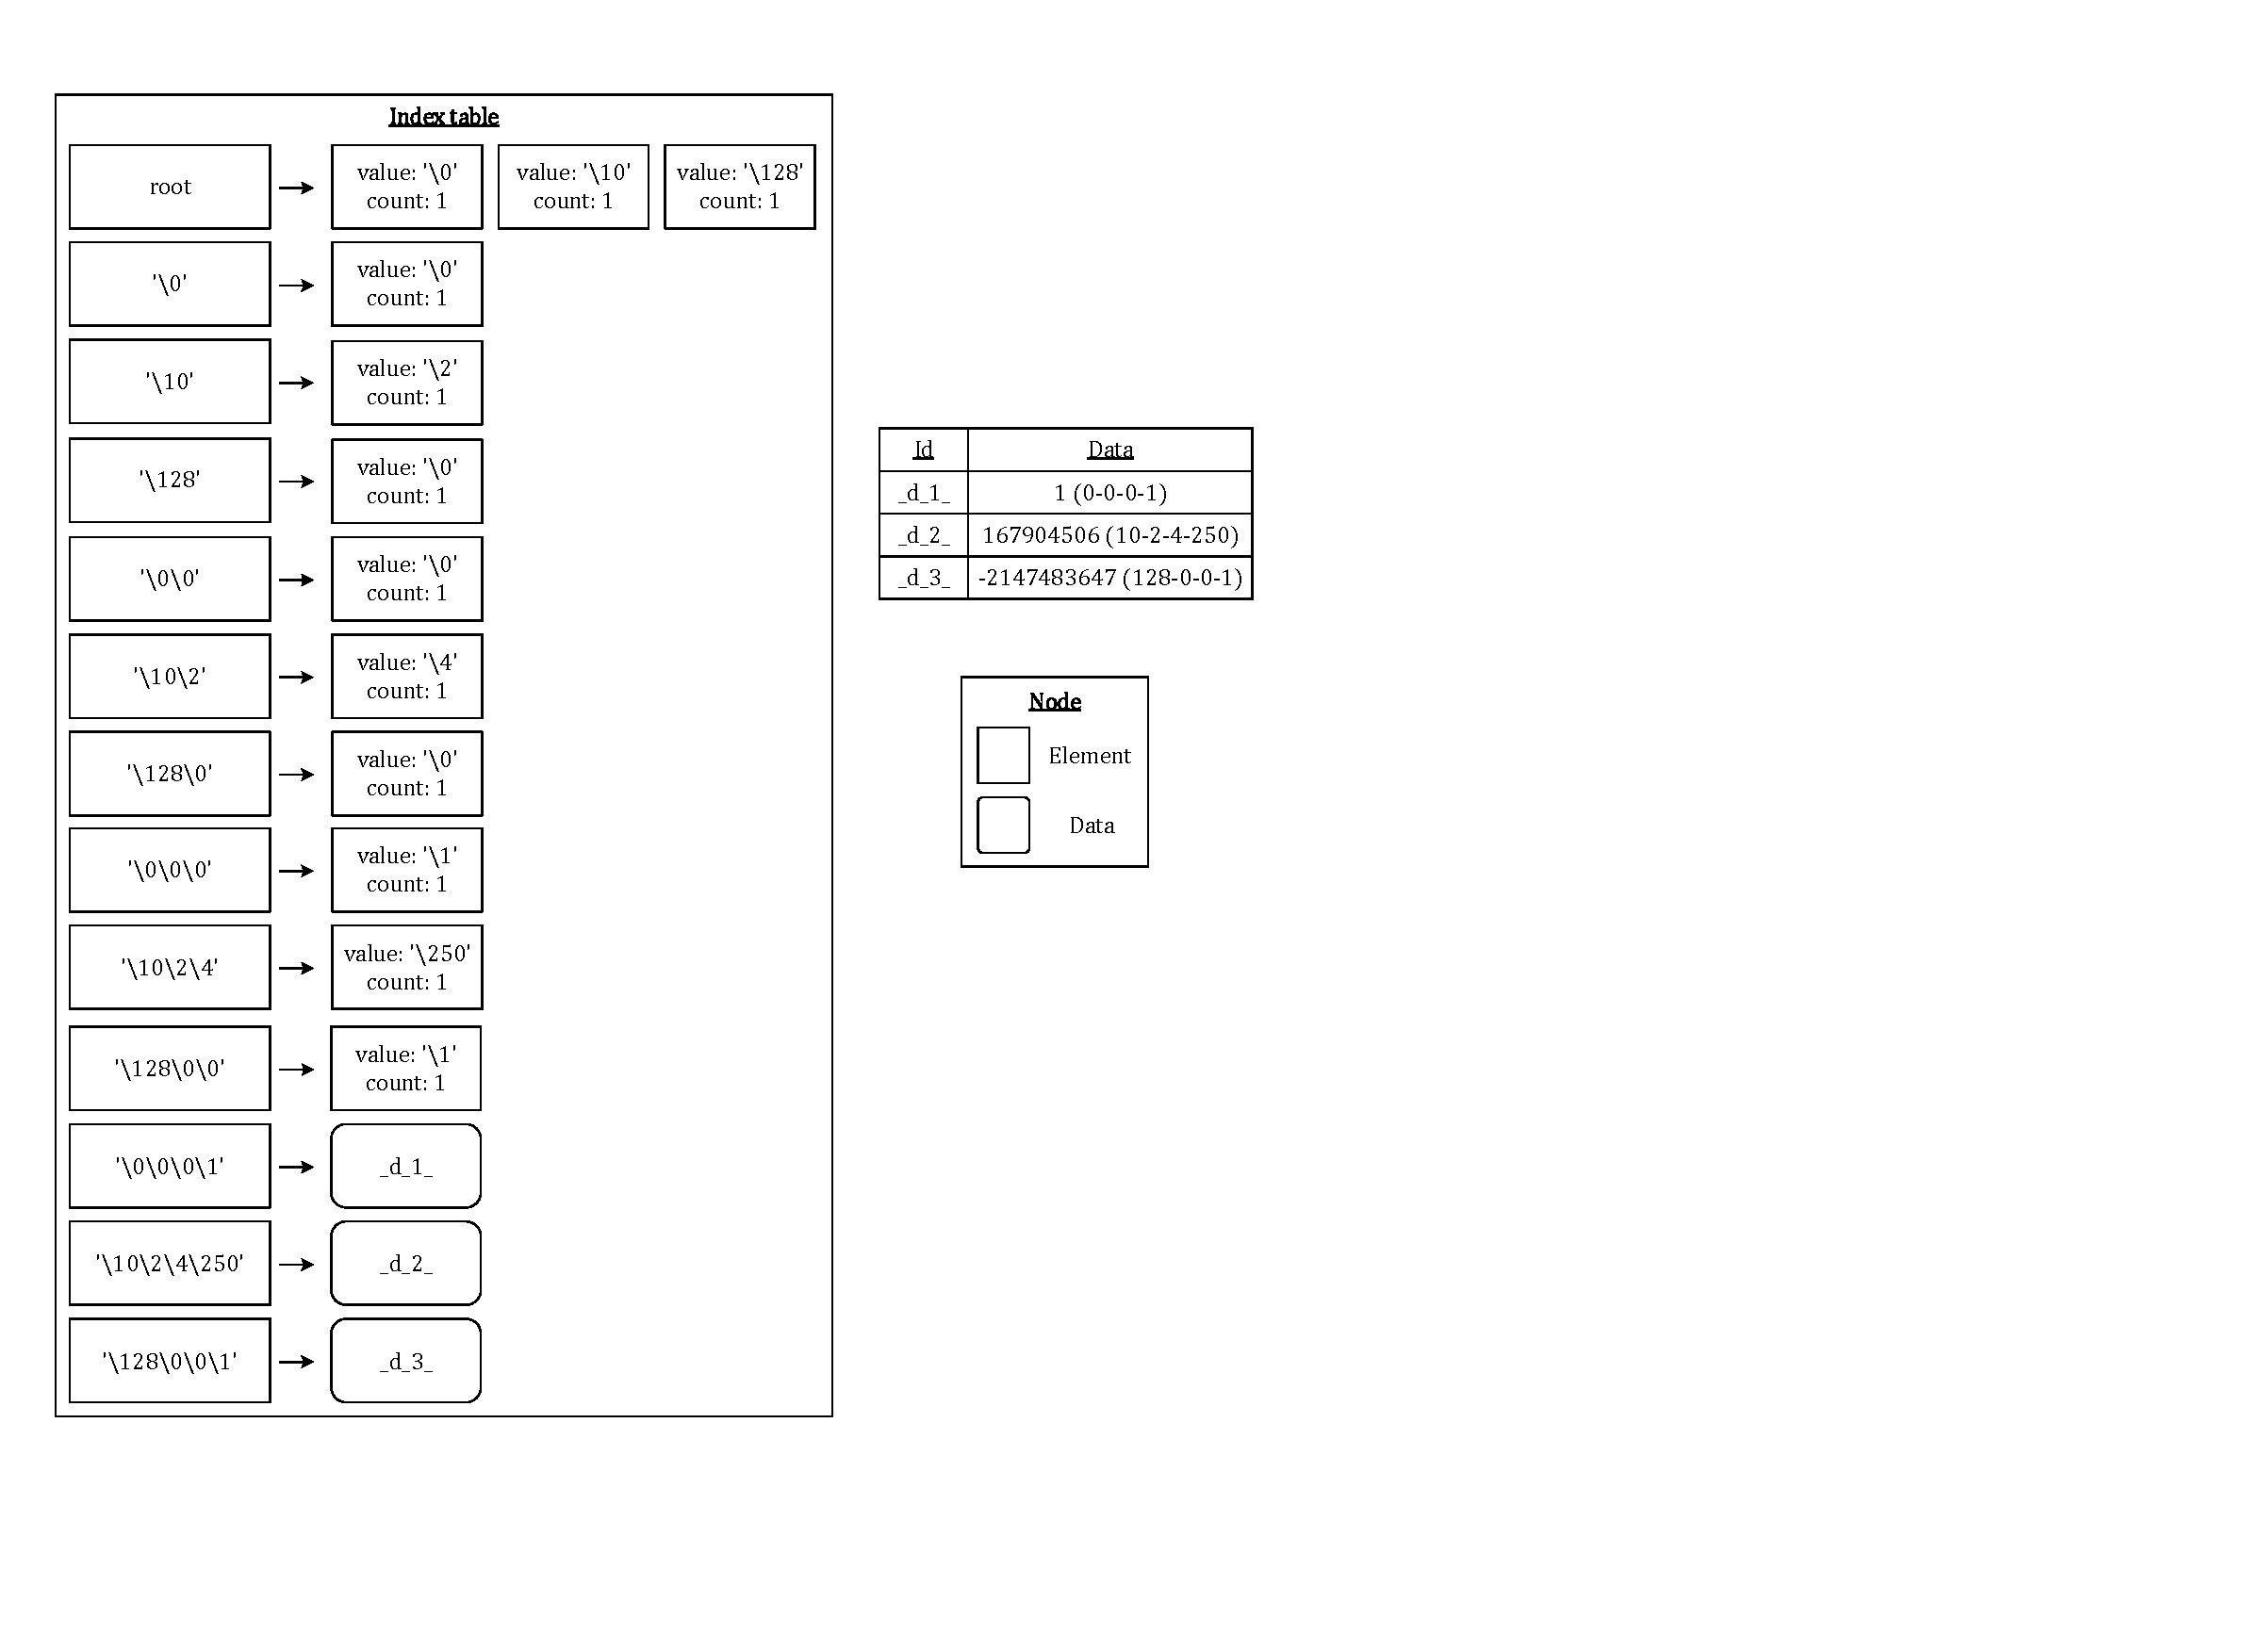
\includegraphics[width=0.8\textwidth]{./algorithm/integer/pic/insertion/example_1_v3.pdf}
\caption{The table after insert a negative value.}
\label{fig:algorithm:integer:insertion:example_1}
\end{figure}

Figure \ref{fig:algorithm:integer:insertion:example_1} shows that even a negative value will store as the same way as the positive value. And time complexity is $O(b)$.



% Deletion section
\subsubsection{Deletion}

Deletion is just do the opposite insertion to remove the byte and decrease the count. Fellow the same rule, if the count become zero, then the node will be remove. The time complexity is also $O(b)$.


% Modification section
\subsubsection{Modification}

The modify flow are similar as \textit{STRING} type, remove the key which don't needed and add the count if the byte is the same. So follow the example in figure \ref{fig:algorithm:integer:insertion:example_1} and modify 167904506 (10-2-4-250) to 2 (0-0-0-2), the table will look like figure \ref{fig:algorithm:integer:modification:example_1} and time complexity is $O(b)$.

\begin{figure}[h]
\centering
%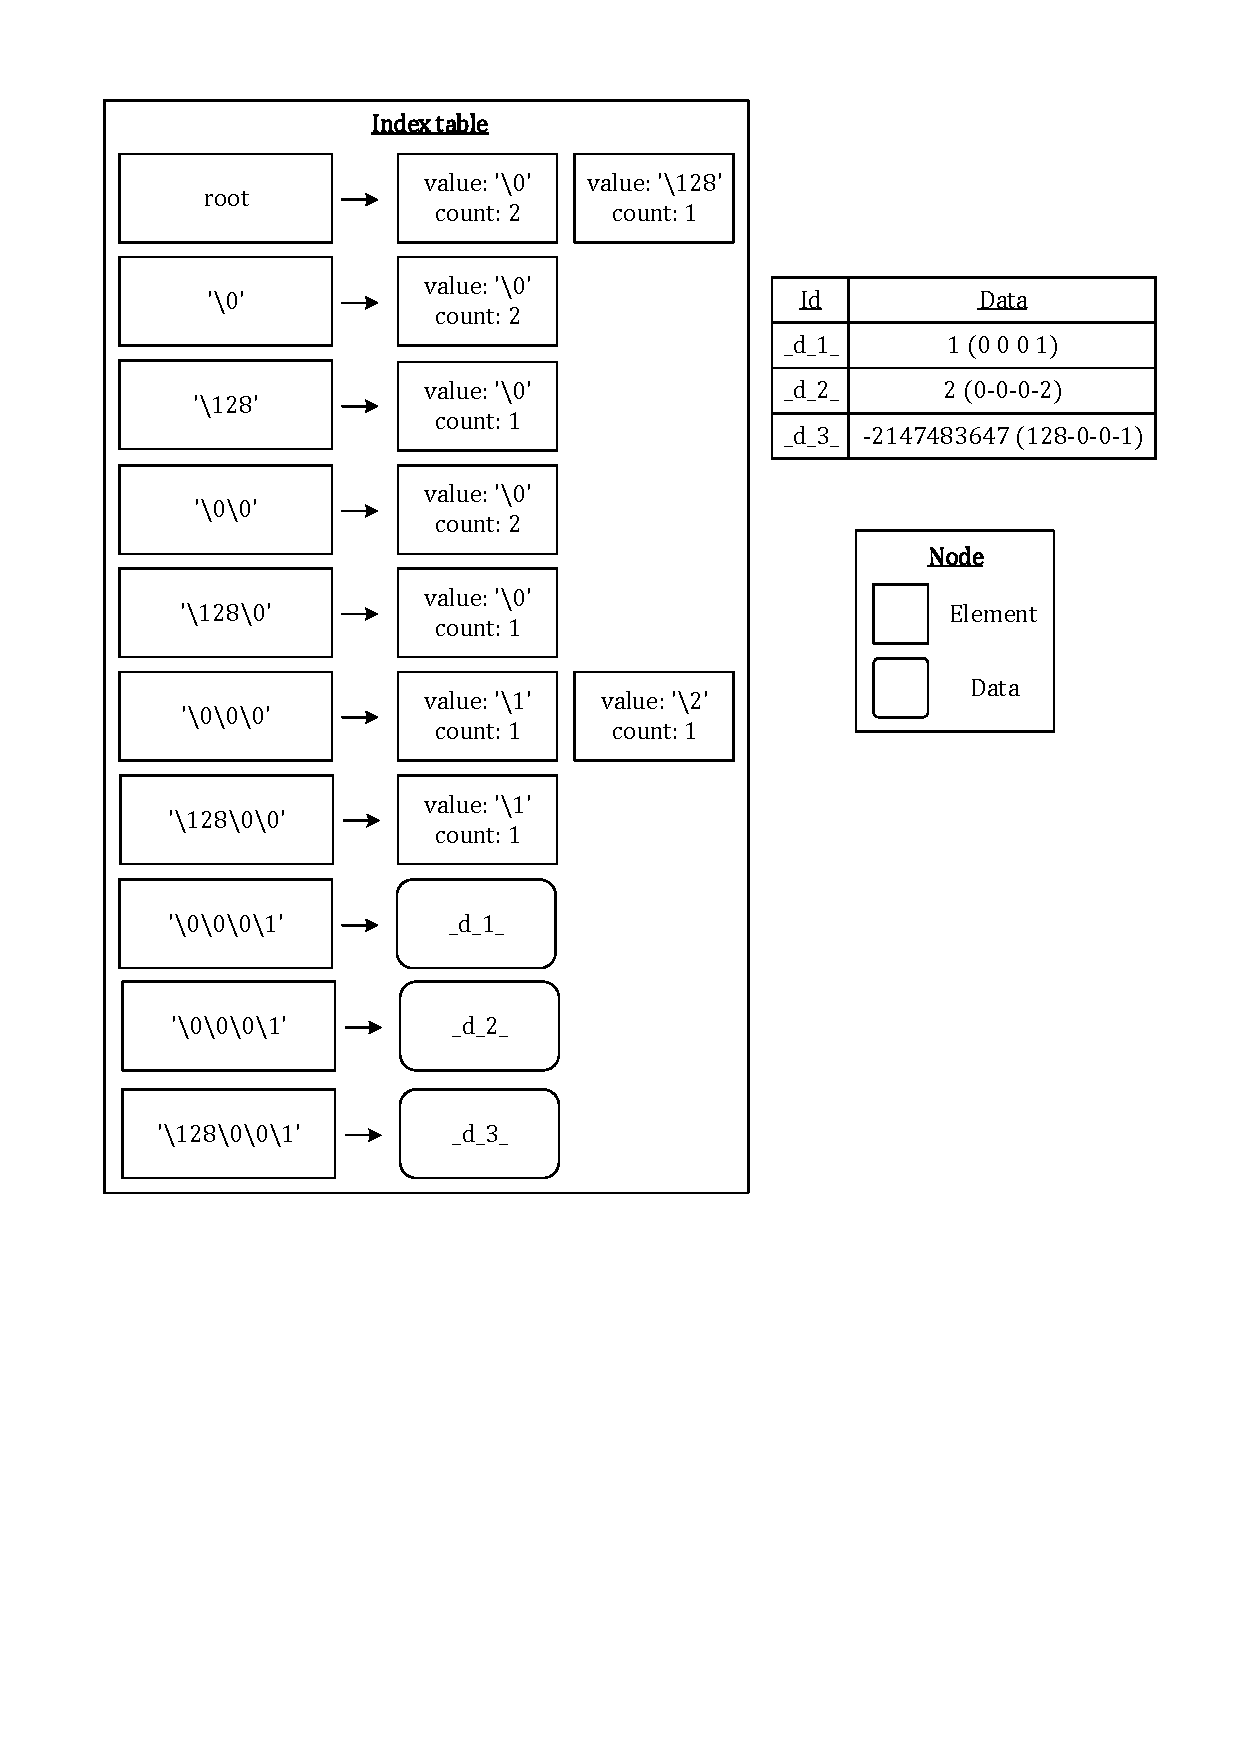
\includegraphics[scale=0.6]{./algorithm/integer/pic/modification/example_1_v3.pdf}
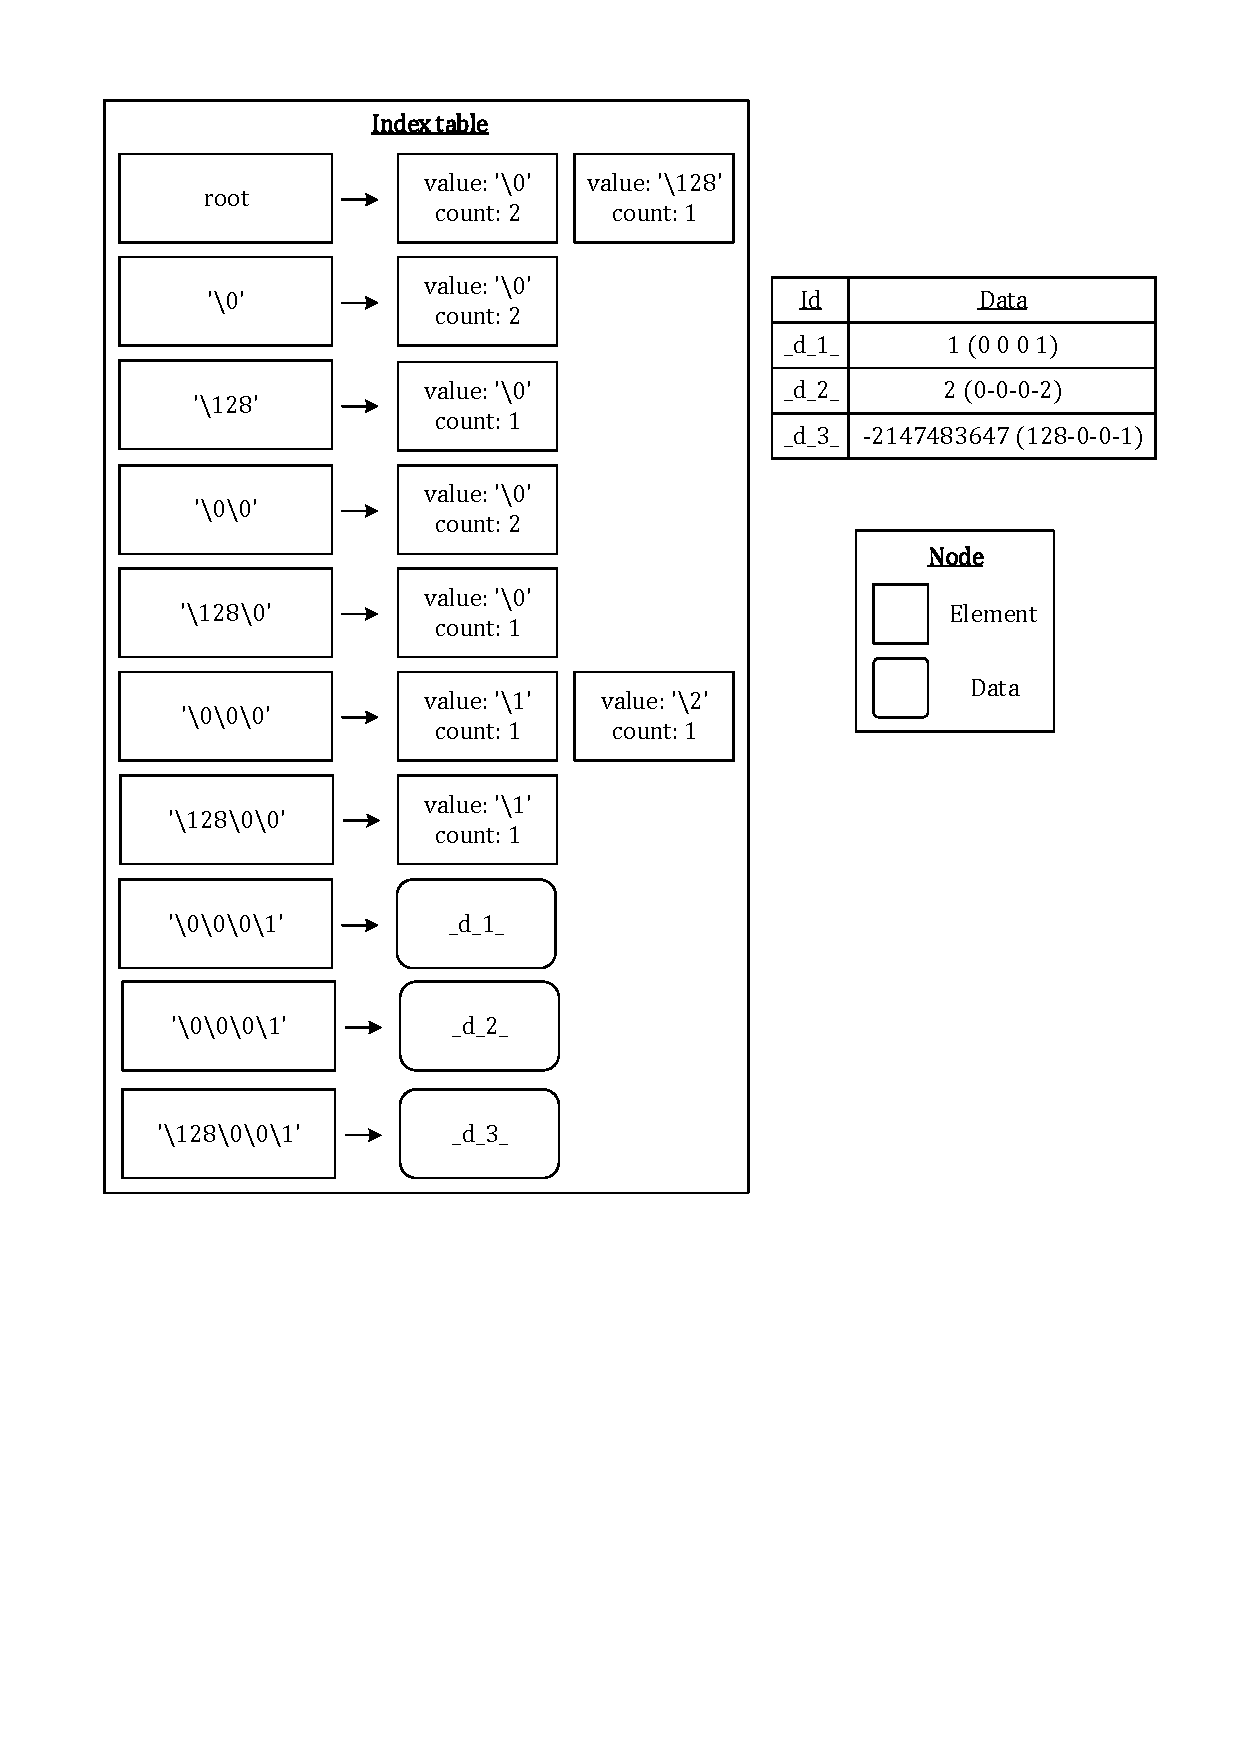
\includegraphics[width=0.8\textwidth]{./algorithm/integer/pic/modification/example_1_v3.pdf}
\caption{The table after modified the value.}
\label{fig:algorithm:integer:modification:example_1}
\end{figure}



% Selection section
\subsubsection{Selection}

Normally the database proves some function for compare the value of searching, so the Li's Hash musts also can do the same thing.

We use figure \ref{fig:algorithm:integer:modification:example_1} as example to demo the selection.

% Selection section enumerate
\begin{enumerate}

% --------------------------------------------------------

% Equal section
\item \textbf{Equal}

Compare the value is very simple. For example if we want to find data is equal to \textit{1 (0-0-0-1)}, we just need to use the key as $'\backslash0\backslash0\backslash0\backslash1'$ to search the index table. This should only take the time as $O(1)$.

% --------------------------------------------------------

% Not equal section
\item \textbf{Not equal}

Because it can't directly use the input value as key. So in this operation, it will start with the root key and parse all the result to find these element node until find the data node, but skip checking the key is as same as the input value. The time complexity be $O(b)$.

% --------------------------------------------------------

% Less than section
\item \textbf{Less than}

The \emph{"Less than"} comparison is similar as \emph{"Not equal"} comparison.

% Less than section description
\begin{description}

% Unsigned section
\item \textbf{Unsigned}

Start from root key, skip all the value which is \textit{"greater than"} the input value of the first byte, for example if the table contain \textit{10-X-X-X}, \textit{15-X-X-X} and \textit{20-X-X-X}, then if the input value is \textit{15-X-X-X}, the result will remain \textit{10-X-X-X} and \textit{15-X-X-X}. After that, search until to the last byte, then check the first byte if it is equal to the first byte of input value, and skip all the last byte which is \textit{"greater than or equal to"} the last byte of input value, otherwise keep all the result.

% Signed section
\item \textbf{Signed}

% Signed section enumerate
\begin{enumerate}

% Input value is a negative value
\item \textbf{Input value is a negative value}

If the input is a negative, then only start from the first byte is \textit{"greater than or equal to"} the inputs' first byte, and skip the key as same as the input.

% Input value is a positive value
\item \textbf{Input value is a positive value}

If the input is a positive, then start from the first byte is \textit{"less than or equal to"} the inputs' first byte and also skip the first byte is \textit{"greater than or equal to"} $\backslash128$ and the key as same as the input.

% Input value is equal to 0.0
\item \textbf{Input value is equal to 0.0}

If the input is zero, then then start from the first byte is \textit{"greater than or equal to"} $\backslash128$.

% End Signed section enumerate
\end{enumerate}

% End Less than section description
\end{description}

The \emph{"Less than or equal to"} comparison is just do the \emph{"Less than"} and \emph{"Equal"} operation and then combine both result for ouput. The time complexity is $O(b)$ for both operation.

% --------------------------------------------------------

% Greater than section
\item \textbf{Greater than}

This comparison flow is same as \emph{"Less than"}, and just need to convert all the \textit{"greater than"} to \textit{"less than"} and \textit{"less than"} to \textit{"greater than"}, the \emph{"Greater than or equal to"} will do the same thing. So time complexities are the same.

% --------------------------------------------------------

% Between section
\item \textbf{Between}

The \emph{"Between"} comparison is combining \emph{"Less than or equal to"} and \emph{"Greater than or equal to"} operation.

% Between section description
\begin{description}

% Unsigned section
\item \textbf{Unsigned}

Start with root key, but only keep the first byte which is only between and equal with the first byte of $minimum$ and $maximum$ input value.

For example if the table contain \textit{5-X-X-X}, \textit{10-X-X-X}, \textit{15-X-X-X}, \textit{20-X-X-X} and \textit{25-X-X-X}, and the input values are \textit{6-X-X-X} and \textit{20-X-X-X}, so \textit{10-X-X-X}, \textit{15-X-X-X} and \textit{20-X-X-X} are the result.

After that, search until to the last byte. Check the first byte if it is equal to the first byte of input value:

% Unsigned section enumerate
\begin{enumerate}[label=\bfseries \arabic*)]

\item When it is equal to the byte of $maximum$ input value, then skip all the last byte which is \textit{"greater than or equal to"} the last byte of $maximum$ input value.

\item When it is equal to the byte of $minimum$ input value, then skip all the last byte which is \textit{"less than or equal to"} the last byte of $minimum$ input value.

\item Otherwise keep all the result.

% End Unsigned section enumerate
\end{enumerate}


% Signed section
\item \textbf{Signed}

In signed integer, there are six cases for the \textbf{Between} operation:

% Signed section enumerate
\begin{enumerate}[label=\bfseries (\arabic*)]

% Case 1
\item \textbf{$minimum$ and $maximum$ are positive}

Use $minimum$ to do the \emph{"Greater than or equal to"}, and do \emph{"Less than or equal to"} by inputting the $maximum$. After that find the common result.

% Case 2
\item \textbf{$minimum$ and $maximum$ are negative}

As same as case \textbf{(1)}.

% Case 3
\item \textbf{$minimum$ is zero and $maximum$ is positive}

Use zero to do the \emph{"Greater than or equal to"}, and do \emph{"Less than or equal to"} by inputting the $maximum$. After that find the common result.

% Case 4
\item \textbf{$minimum$ is negative and $maximum$ is zero}

Use $minimum$ to do the \emph{"Greater than or equal to"}, and do \emph{"Less than or equal to"} by inputting the zero. After that find the common result.

% Case 5
\item \textbf{$minimum$ is negative and $maximum$ is positive}

Cut this into two part, the negative to zero part will do the \textbf{(4)}, another part will do \textbf{(3)}, after that find the common result.

% Case 6
\item \textbf{$minimum$ is positive value and $maximum$ are negative value}

This case should never happend because of the program should show warning message if the user really inputed like this.

% End Signed section enumerate
\end{enumerate}

The time complexity is $O(b)$.

% End Between section description
\end{description}
% --------------------------------------------------------

% End Selection section enumerate
\end{enumerate}



% Summary section
\subsubsection{Summary}

Table \ref{table:algorithm:integer:summary:time_complexity} is the summary the time complexity of each opration in \textit{INTEGER} type.

\begin{table}[h]
\centering
\caption{Time complexity for \textit{INTEGER} type.}
\label{table:algorithm:integer:summary:time_complexity}
\begin{tabular}{|c|c|}

\hline
\multicolumn{1}{|c|}{Operation} &
\multicolumn{1}{c|}{\tabincell{c}{
Time complexity \\ ($b$: The byte length of data, $b$ = 8)
}} \\

\hline
\multicolumn{1}{|c|}{Insert} &
\multicolumn{1}{c|}{$O(b)$)} \\

\hline
\multicolumn{1}{|c|}{Modify} &
\multicolumn{1}{c|}{$O(b)$)} \\

\hline
\multicolumn{1}{|c|}{Delete} &
\multicolumn{1}{c|}{$O(b)$)} \\

\hline
\multicolumn{1}{|c|}{Equal} &
\multicolumn{1}{c|}{$O(1)$} \\

\hline
\multicolumn{1}{|c|}{\tabincell{c}{Equal (muti-value)}} &
\multicolumn{1}{c|}{$O(1)$} \\

\hline
\multicolumn{1}{|c|}{Not equal} &
\multicolumn{1}{c|}{$O(b)$)} \\

\hline
\multicolumn{1}{|c|}{\tabincell{c}{Not equal (muti-value)}} &
\multicolumn{1}{c|}{$O(b)$)} \\

\hline
\multicolumn{1}{|c|}{Less than} &
\multicolumn{1}{c|}{$O(b)$)} \\

\hline
\multicolumn{1}{|c|}{Less than or equal} &
\multicolumn{1}{c|}{$O(b)$)} \\

\hline
\multicolumn{1}{|c|}{Greater than} &
\multicolumn{1}{c|}{$O(b)$)} \\

\hline
\multicolumn{1}{|c|}{Greater than or equal} &
\multicolumn{1}{c|}{$O(b)$)} \\

\hline
\multicolumn{1}{|c|}{Between} &
\multicolumn{1}{c|}{$O(b)$)} \\

\hline
\end{tabular}
\end{table}


\clearpage
